%-----------------------------------------------------------------
%	IMPLEMENTATION
%	!TEX root = ./../main.tex
%-----------------------------------------------------------------
\section{Implementation using MATLAB}
Before starting the actual implementation, we need realistic physical values for the different parameters involved in the problem.

For the physical parameters of the car, we will use the specifications of a Mercedes-Benz C-Class S203 (as seen in figure \ref{fig:car-sideview}): $L_{1} = \SI{2.715}{\m}$, $L_{2} = \SI{1.169}{\m}$. We will assume the distance from the trailer axle to the hitch is $L_{3} = \SI{1.2}{\m}$.

\begin{figure}[H]
	\centering
	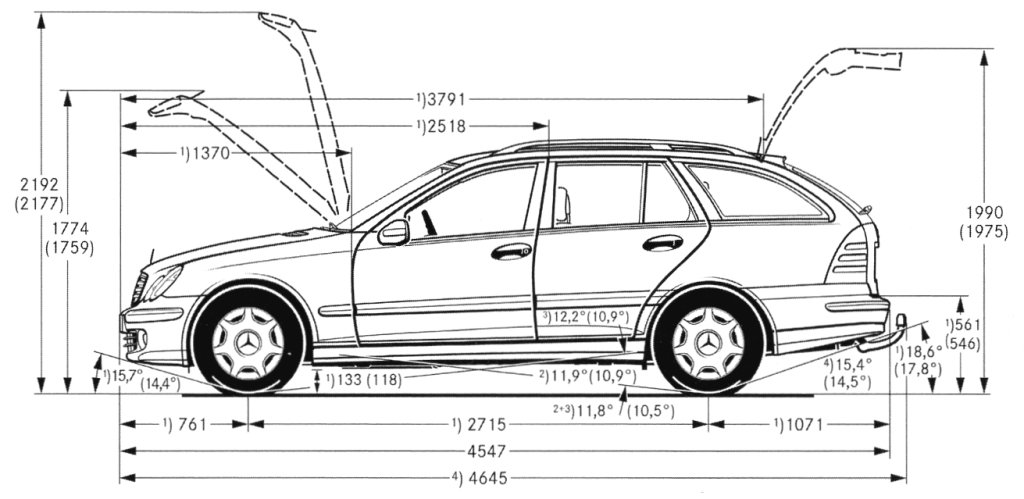
\includegraphics[width=0.95\textwidth]{images/S203_Seitenansicht}
	\caption{Side view diagram of a Mercedes-Benz CLC S203 AMG}
	\label{fig:car-sideview}
\end{figure}

%-----------------------------------------------------------------
\subsection{Programming the Controller}
The first need we need to do is to define some of the physical parameters of the system defined in table~\ref{tab:parameters}, this is shown in snippet~\ref{sn:physical} below:
\begin{lstlisting}[language=matlab, label=sn:physical, caption=Physical parameters for the model]
%% Parameters
% Reference angle
r = 0.25;
% Initial condition in degree
phi_0 = r + 0.1;
% Velocity in meters per second
V = 3.0;
% Example for Mercedes-Benz CLC S203 AMG in meters
L1 = 2.715;
L2 = 1.169;
L3 = 1.2;
\end{lstlisting}

As discussed in \cref{sec:intro-msct}, the eigenvalues of the system matrix, $A$, (equal to the poles of the transfer function) determine stability. In our system \eqref{eq:controler-system} we see that $A$ is positive; thus the system is unstable. The parameters to model the controller are defined in snippet~\ref{sn:model} below:
\begin{lstlisting}[language=matlab, label=sn:model, caption=Basic parameters to model the controller, firstnumber=13]
%% Model
A = V/L3;
B = V/L1*(1+L2/L3);
C = 1;
D = 0;
\end{lstlisting}

One of the first things we want to do is analyse whether the open-loop system (without any control) is stable. To observe what happens to this unstable system when there is a non-zero initial condition, we define the state space using \inline{sys = ss(A,B,C,0)} and then we simulate the output time response $y(t)$ of dynamic system with input $u(t)$ using the function \inline{lsim()}. This implementation can be seen in snippet~\ref{sn:open-loop} below:
\begin{lstlisting}[language=matlab, label=sn:open-loop, caption=Method to calculate open-loop response to non-zero initial condition, firstnumber=20]
%% Calculate open-loop response to non-zero initial condition

% Time in seconds
t = 0:0.01:10;
% Input
u = zeros(size(t))*r;
% Create state space object
sys = ss(A,B,C,0);

% Calculate open-loop response to non-zero initial condition
[y,t,x] = lsim(sys,u,t,phi_0);

% Plot the response
figure(1)
	plot(t,y)
	hold on
	plot(t,u)
	str_num = num2str(phi_0);
	str = strcat('Open-Loop Response to Non-Zero Initial Condition \phi_0=', str_num);
	title(str)
	xlabel('Time (sec)')
	ylabel('\phi (rad)')
	legend('Open-loop response', 'Reference')
	hold off
\end{lstlisting}

In figure \ref{fig:curve-open-loop} below we can see the uncontrolled behaviour of the system when there are no closed-loop poles (i.e., open-loop response). It's remarkable how quickly the jackknifing phenomenon occurs.
\begin{figure}[H]
	\centering
	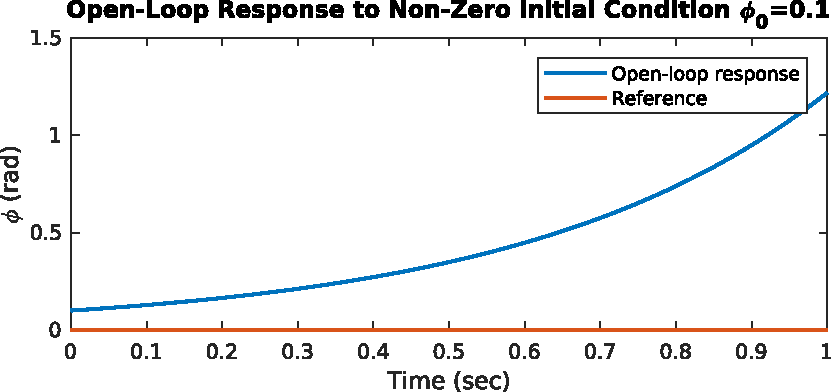
\includegraphics[width=0.7\textwidth]{images/curve-open-loop}
	\caption{Open-Loop response to non-zero initial condition driving backwards with a trailer}
	\label{fig:curve-open-loop}
\end{figure}

It is also worth noting that just as we expected from \eqref{eq:stability}, when $V < 0$ (using \inline{V = -3.0;} for instance) the system is stable, as seen in figure~\ref{fig:curve-open-loop-stable} below. In the figure, it can be clearly seen how when the car moves forward, the angle $\phi$ is corrected in a matter of seconds and then trailer flawlessly follows the car.
\begin{figure}[H]
	\centering
	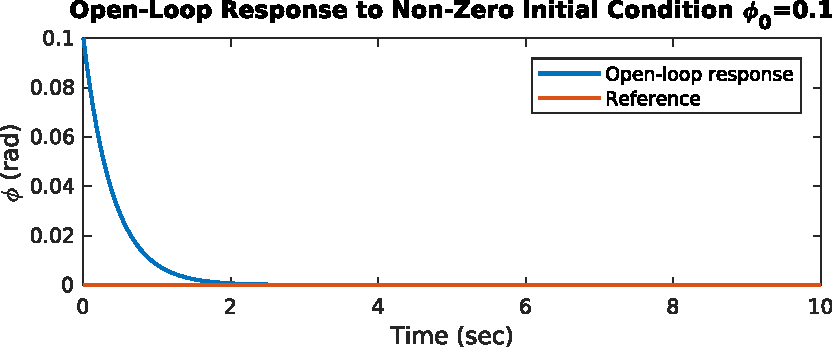
\includegraphics[width=0.73\textwidth]{images/stable-open-loop}
	\caption{Open-Loop response to non-zero initial condition driving forwards with a trailer}
	\label{fig:curve-open-loop-stable}
\end{figure}

%----------------------------------
Now that we know how the system behaves when there is no actual controller, let's see what happens when we introduce a closed-loop pole to control the system. We will work with several reference trajectories (discussed in \cref{sec:curves}) to see how the controller can handle different scenarios.

The major difference between this method and the previous one is that we now  build the controller for the system using a pole placement approach and assuming we have a full-state feedback system, meaning that all state variables are known to the controller at all times.

We use the function \inline{place()} to find the state-feedback gain, $K$, which will provide the desired closed-loop poles. Then we define the state space using \inline{sys_cl = ss(A-B*K,B,C,0);} and simulate the output time response $y(t)$ of dynamic system with input $u(t)$ using the function \inline{lsim()}, as seen in snippet~\ref{sn:closed-loop}.

One may see that we use a $\bar{N}$ factor in the calculation of the time response. We use the function \inline{rscale(sys,K)} to compute the desired $\bar{N}$ like presented in \cref{sec:controllerdesign}.

\begin{lstlisting}[language=matlab, label=sn:closed-loop, caption=Method to calculate closed-loop response to non-zero initial condition, firstnumber=44]
%% Calculate closed-loop response to non-zero initial condition

% Time in seconds
t = 0:0.01:60;
% Inputs
u = curve1(t, 0.35); % Standard curve
% u = curve2(t, 0.4); % U turn
% u = curve3(t, 0.65); % Sharp curve
% u = curve4(t, 0.4); % S shape

% Apply pole placement
K = place(A,B,-0.73);
% State space
sys_cl = ss(A-B*K,B,C,0);
% Calculate scaling factor
Nbar = rscale(sys,K);

% Calculate closed-loop response to non-zero initial condition
[y_cl,t,x_cl] = lsim(sys_cl,Nbar*u,t,phi_0);

% Plot the response
figure(2)
	plot(t,y_cl)
	hold on
	plot(t,u)
	str = strcat('Closed-Loop Response to Non-Zero Initial Condition \phi_0=', str_num);
	title(str)
	xlabel('Time (sec)')
	ylabel('\phi (rad)')
	legend('Closed-loop response', 'Reference')
	hold off
\end{lstlisting}

This implementation of a controller is the one previously illustrated in figure~\ref{fig:gain-schedule}.

%-----------------------------------------------------------------
\subsection{Controlling the Trailer on Different Curves}\label{sec:curves}
In this part we will see how the controller performs in terms of reaction time and fidelity with different trajectories. In particular we will work with (a) a short sharp curve, (b) a $U$ turn, and (c) an $S$-shaped curve.

%----------------------------------
\subsubsection*{Standard Curve}
In figure~\ref{fig:curve1a} we can see the shape of the trajectory followed by the car-trailer system, and in figure~\ref{fig:curve1b} we can see how the response of the controller to the input trajectory (defined in snippet~\ref{sn:curve1b}).

\begin{figure}[H]
	\centering
	\subfloat[Diagram of the curve]{%
		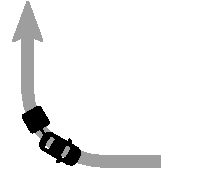
\includegraphics[height=0.2\textwidth]{images/curve1-diagram}%
		\label{fig:curve1a}%
		}%
	\hspace{0.5cm}%
	\subfloat[Closed-loop response of the controller]{%
		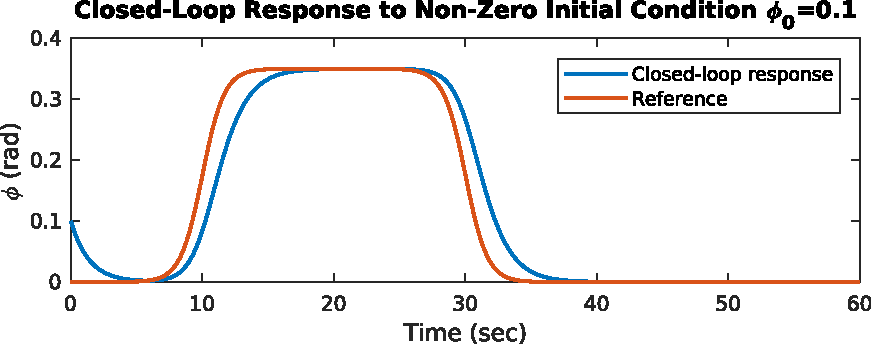
\includegraphics[height=0.25\textwidth]{images/control1-plot}%
		\label{fig:curve1b}%
		}%
	\caption{Diagram and control of the car-trailer system in a short, sharp curve}
\end{figure}

\begin{lstlisting}[language=matlab, label=sn:curve1b, caption=Function used to simulate a standard curve]
function [ x ] = curve1( t, height)
    steep = 2;
    n = length(t);

    x_1 = logistic(height, steep, linspace(-6,6,floor(n/3)), 0);
    x_2 = flip(x_1);

    x = [ x_1 height x_2 zeros(1,floor(n/3)) ];
end
\end{lstlisting}

This curve, along with a straight line, are the basis of basically all possible trajectories a car-trailer system can make whilst parking.

%----------------------------------
\subsubsection*{$U$-Turn Curve}
A $U$ turn simply consists on steering the wheel a longer time to the standard curve pr

In figure\ref{fig:curve2a} we can see the shape of the trajectory followed by the car-trailer system, and in figure~\ref{fig:curve2b} we can see how the response of the controller to the input trajectory (defined in snippet~\ref{sn:curve2}).

\begin{figure}[H]
	\centering
	\subfloat[Diagram of the curve]{%
		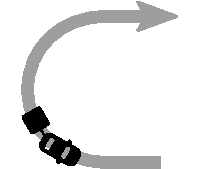
\includegraphics[height=0.2\textwidth]{images/curve2-diagram}%
		\label{fig:curve2a}%
		}%
	\hspace{0.5cm}%
	\subfloat[Closed-loop response of the controller]{%
		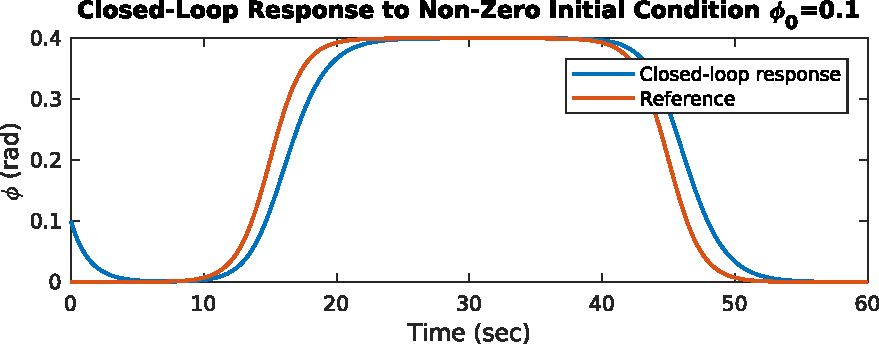
\includegraphics[height=0.25\textwidth]{images/control2-plot}%
		\label{fig:curve2b}%
		}%
	\caption{Diagram and control of the car-trailer system in a $U$ turn}
\end{figure}
\begin{lstlisting}[language=matlab, label=sn:curve2, caption=Function used to simulate a $U$ turn]
function [ x ] = curve2( t, height)
	steep = 2;
	n = length(t);

	x_1 = logistic(height, steep, linspace(-6,6,floor(n/2)), 0);
	x_2 = flip(x_1);

	x = [x_1 height x_2];
end
\end{lstlisting}

%----------------------------------
\subsubsection*{Short, Sharp Curve}
In figure~\ref{fig:curve3a} we can see the shape of the trajectory followed by the car-trailer system, and in figure~\ref{fig:curve3b} we can see how the response of the controller to the input trajectory (defined in snippet~\ref{sn:curve3b}).

\begin{figure}[H]
	\centering
	\subfloat[Diagram of the curve]{%
		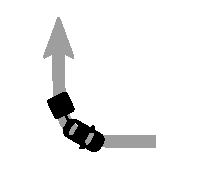
\includegraphics[height=0.2\textwidth]{images/curve3-diagram}%
		\label{fig:curve3a}%
		}%
	\hspace{0.5cm}%
	\subfloat[Closed-loop response of the controller]{%
		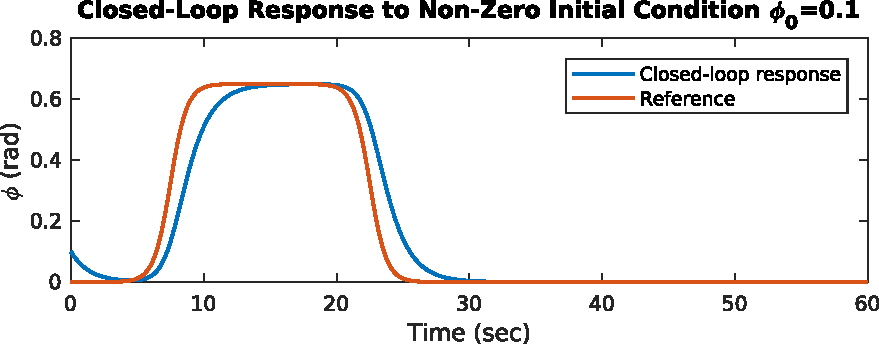
\includegraphics[height=0.25\textwidth]{images/control3-plot}%
		\label{fig:curve3b}%
		}%
	\caption{Diagram and control of the car-trailer system in a short, sharp curve}
\end{figure}

\begin{lstlisting}[language=matlab, label=sn:curve3b, caption=Function used to simulate a short sharp curve]
function [ x ] = curve1( t, height)
	steep = 2;
	n = length(t);

	x_1 = logistic(height, steep, linspace(-6,6,floor(n/4)), 0);
	x_2 = flip(x_1);

	x = [ x_1 height x_2 zeros(1,floor(n/2)) ];
end
\end{lstlisting}

%----------------------------------
\subsubsection*{$S$-Shaped Curve}
In figure~\ref{fig:curve4a} we can see the shape of the trajectory followed by the car-trailer system, and in figure~\ref{fig:curve4b} we can see how the response of the controller to the input trajectory (defined in snippet~\ref{sn:curve4}).

\begin{figure}[H]
	\centering
	\subfloat[Diagram of the curve]{%
		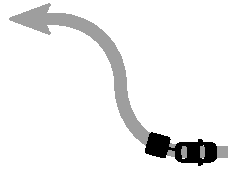
\includegraphics[height=0.2\textwidth]{images/curve4-diagram}%
		\label{fig:curve4a}%
		}%
	\hspace{0.5cm}%
	\subfloat[Closed-loop response of the controller]{%
		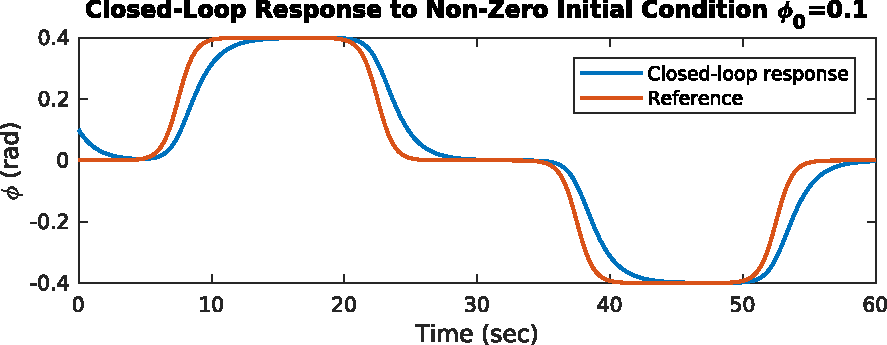
\includegraphics[height=0.25\textwidth]{images/control4-plot}%
		\label{fig:curve4b}%
		}%
	\caption{Diagram and control of the car-trailer system in a $S$-shaped curve}
\end{figure}
\begin{lstlisting}[language=matlab, label=sn:curve4, caption=Function used to simulate an $S$-shaped curve]
function [ x ] = curve3( t, height )
	steep = 2;
	n = length(t);

	x_1 = logistic(height, steep, linspace(-6,6,floor(n/4)), 0);
	x_2 = flip(x_1);
	x_3 = [ x_1 x_2 ];
	x_4 = -x_3;

	x = [ x_3 0 x_4 ];
end
\end{lstlisting}

%-----------------------------------------------------------------
\subsection{Issues with the Model}

Main problem about this model is that it is a continuous model which cannot be implemented on a chip without modification. One needs to discretise it. There are several options to do so, each having advantages and disadvantages. One could think about creating a continuous model with continuous model and afterwards doing the discretisation. Another approach would be just to discretise the model and create a discrete version of the controller. These two approaches are not equivalent. Obviously, the first one is more powerful because it will provide insights into the system behaviour for all times $t$ whereas the second one only yield information for the sampling instances $kT$. The advantage of this method is that it is easier to apply.

Another problem is that the model is obtained by linearisation about the operation point $\SI{0}{\degree}$. One improvement would be to use a gain-scheduling controller which is also linear. This group of controller is often applied to nonlinear models. It selects the gain according to some strategy. This strategy e.g. can be time-varying or depended on the state of the system. In our case we would prefer a state dependent scheduler since our system behaves linearly in small regions for different operating points: $[-\SI{40}{\degree},\SI{40}{\degree}]$. For implementation we would need to linearise the model for all these operating points with a sufficient small step size. However, to show feasibility and solvablity of the problem it is sufficient to linearise about one operation point. 
